\chapter{Infraestructura}
En esta sección se describe con cierto detalle las herramientas, estándares y bibliotecas que hemos usado directamente en el desarrollo de este TFG.
\section{HTML5}
Este nuevo estándar incorpora una series de APIs accesibles desde JavaScript que surgen para dotar de funcionalidad nativa a la Web sin necesidad de utilizar plugins externos. Los distintos ingredientes asociados a HTML5 \cite{html5} los describimos en las siguientes secciones.
\subsection{Canvas}
El elemento \texttt{<canvas>} \cite{canvas}  permite trabajar con gráficos orientados a píxel (no vectorial) dentro de la web sin la necesidad de emplear programas externos. Dispone de varios métodos que permiten realizar múltiples tareas de carácter gráfico que explicamos a continuación.
\subsubsection*{Context 2d}
Es el punto de partida para utilizar las propiedades de canvas. Es necesario acceder a la etiqueta canvas existente en el documento para obtener el contexto.
\\El contexto puede ser 2D y 3D dependiendo del tipo de elementos que se quieren dibujar.
\begin{lstlisting}[
caption=Acceso al contexto de Canvas.]
 var canvas = document.getElementById('tutorial');
 var ctx = canvas.getContext('2d');
\end{lstlisting}
\subsubsection*{Formas Disponibles}
Por medio del contexto tenemos acceso a un conjunto de métodos que permiten dibujar primitivas predefinidas,que se explican a continuación.
\begin{enumerate}
\item Trazos
  \begin{itemize}
      \item \texttt{beginPath():} Marcan el inicio de un nuevo trazo.
      \item \texttt{closePath():} Marcan el final del trazo definido.
      \item \texttt{stroke():} Dibuja el contorno de la forma.
      \item \texttt{fill():} Dibuja una forma solida rellenando el área del trazo.
  \end{itemize}
\item Líneas: La función \texttt{lineTo(x,y)} permite dibujar lineas. Toma como punto de partida el ultimo punto conocido y como  punto final la coordenada(x,y) que se le pasa.
\item Movimiento: La función \texttt{moveTo(x, y)} permite moverse a un punto del lienzo para empezar a dibujar a partir de él.
\begin{figure}[!h]
\begin{center}
   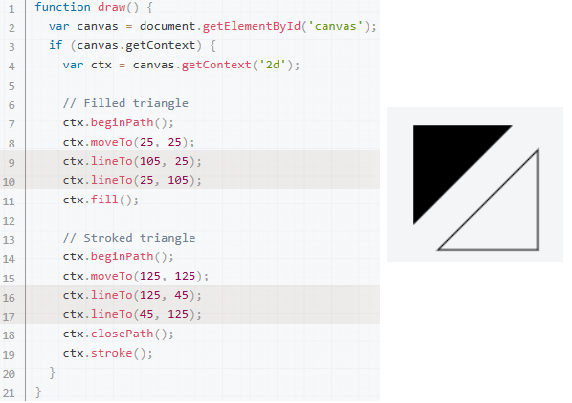
\includegraphics[width=0.8\linewidth]{Figures/lineas_Canvas}
  \decoRule
  \caption[Ejemplo del dibujo de un trazo]{Ejemplo del dibujo de un trazo.}
\label{fig:lineas_Canvas}
\end{center}
\end{figure}
\item Rectángulos
  \begin{itemize}
      \item \texttt{fillRect(x, y, width, height):} Dibuja un rectángulo relleno.
      \item \texttt{strokeRect(x, y, width, height):} Dibuja el contorno de un rectángulo.
      \item \texttt{clearRect(x, y, width, height):} Borra el área rectangular especificada.
  \end{itemize}
\begin{figure}[!h]
\begin{center}
   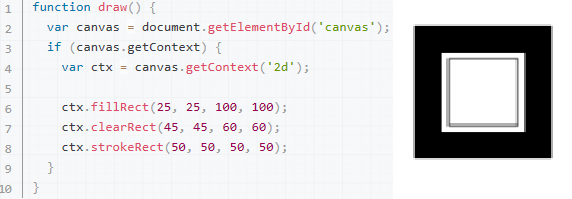
\includegraphics[width=0.8\linewidth]{Figures/Rectangulos_Canvas}
  \decoRule
  \caption[Ejemplo rectángulos canvas]{Ejemplo rectángulos canvas.}
\label{fig:Rectangulos_Canvas}
\end{center}
\end{figure}
\item Arcos: Por medio de la función \texttt{arc(x,y,radio,angInit,angFin,true)} se dibuja una circunferencia o media circunferencia. Para realizar este proceso establece como centro las coordenadas (x,y) ,su tamaño depende del radio que se especifique y por ultimo establecemos el ángulo inicial y final que queremos.
\end{enumerate}
\subsubsection*{Estilos y Colores}
Para poder aplicar colores a los dibujos que se crean tenemos a nuestra disposición dos propiedades que podemos usar:
\begin{itemize}
\item \texttt{fillStyle:} Establece el color de relleno de la figura.
\item \texttt{strokeStyle:} Establece el color del contorno de la figura.
\end{itemize}
Además de dibujar formas opacas en el lienzo,también podemos dibujar formas semitransparentes (o translúcidas). Esto se realiza  estableciendo la propiedad globalAlpha o asignando un color semitransparente al estilo de trazo y/o de relleno.
\begin{itemize}
\item \textbf{globalAlpha:} Aplica el valor de transparencia especificado a todas las formas futuras del lienzo.El valor debe estar entre 0,0 (totalmente transparente) y 1,0 (completamente opaco).
\end{itemize}
Por otra parte se puede establecer el estilo de las lineas que componen las figuras, por medio las siguientes propiedades:
\begin{itemize}
\item \texttt{lineWidth:} Establece el ancho de las lineas.
\item \texttt{lineCap:} Establece el aspecto de los extremos de las lineas.Estos atributos pueden ser: butt(extremos cuadrado),round(extremos redondeados) y square()
\item \texttt{lineJoin:} Establece el aspecto de las esquinas donde se encuentran las lineas.Estos atributos pueden ser: round() , bevel() y miter().
\end{itemize}
\subsubsection*{Texto}
Permite generar cadenas de texto dentro de canvas por medio del método \texttt{fillText(text,x,y)} que recibe como parámetro el texto y la coordenada donde se dibujarán, figura \ref{fig:Texto_Canvas}.
\begin{itemize}
\item \texttt{fillText(text,x,y):} Dibuja el texto dado en las coordenadas(x,y) del lienzo.
\item \texttt{strokeText(text,x,y):} Dibuja el texto dado en las coordenadas(x,y) del lienzo sin relleno.
\end{itemize}
Ademas permite establecer el estilo del texto por medio de las siguientes propiedades:
\begin{itemize}
\item \texttt{font:} Estilo del texto que se utiliza al dibujar el texto.Los valores permitidos son similares a las propiedades CSS font.
\item \texttt{textAlign:} Alinea el texto.Los valores disponibles son: start,end,left,rigth o center.
\item \texttt{direction:} Direccionalidad del texto.
\end{itemize}
\begin{figure}[!h]
\begin{center}
   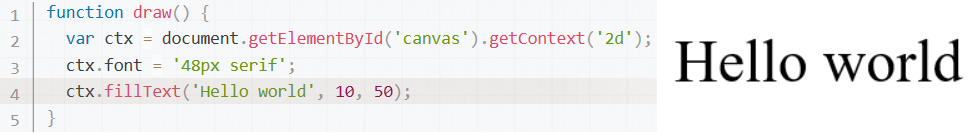
\includegraphics[width=0.8\linewidth]{Figures/Texto_Canvas}
  \decoRule
  \caption[Ejemplo texto canvas]{Ejemplo texto canvas.}
\label{fig:Texto_Canvas}
\end{center}
\end{figure}
\subsubsection*{Imágenes}
Para importar imágenes en el lienzo es necesario obtener la referencia de un objeto HTMLImageElement como fuente y dibujarla en el lienzo por medio de la función \texttt{drawImage()}.  
\\Para cargar una imagen externa es necesario genera un objeto HTMLImageElement por medio de JavaScript. Para ello, utilizamos el constructor \texttt{Image()} en el que definimos la dirección de la imagen en el atributo \texttt{src} y por medio del método \texttt{load} nos aseguraremos que la carga se ha completado.
\\Tras obtener la referencia a nuestra imagen podemos utilizar los método disponibles para cargar las imágenes en el lienzo.A continuación,se muestra las variantes del método ya que se encuentra sobrecargado. 
\begin{itemize}
\item \texttt{drawImage(img,x,y):} Dibuja la imagen especifica en las coordenadas(x,y) del lienzo.
\item \texttt{drawImage(image, x, y, width, height):} Dibuja la imagen específica en las coordenadas(x,y) estableciendo la escala en la que se dibuja por medio de los parámetros \texttt{width} y \texttt{height}, figura \ref{fig:ImagenScale_Canvas}.
\begin{figure}[!h]
\begin{center}
   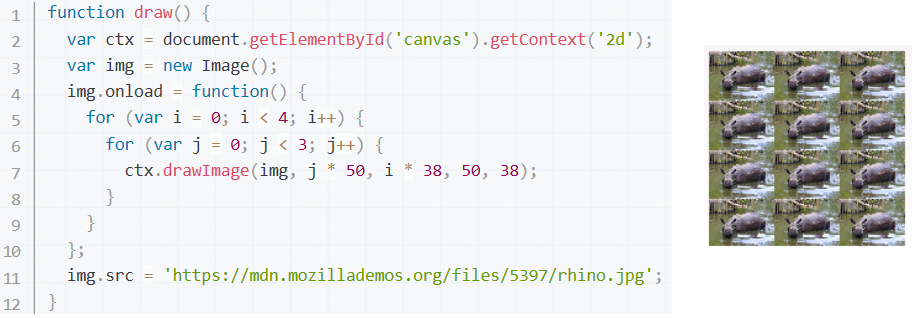
\includegraphics[width=0.8\linewidth]{Figures/ImagenScale_Canvas}
  \decoRule
  \caption[Ejemplo escalado de imagen canvas.]{Ejemplo escalado de imagen canvas.}
\label{fig:ImagenScale_Canvas}
\end{center}
\end{figure}
\item \texttt{drawImage(image, sx, sy, sWidth, sHeight, dx, dy, dWidth, dHeight):} Dada una imagen, esta función toma el área de la imagen de origen por el rectángulo cuya esquina superior izquierda es (sx,sy) y cuya anchura y la altura son \texttt{sWidth} y \texttt{sHeight}, colocándolo en el lienzo en las coordenadas(dx,dy) y escalado por medio de \texttt{dWidth} y \texttt{dHeight}, figura \ref{fig:ImagenRecorte_Canvas}.
\begin{figure}[!h]
\begin{center}
   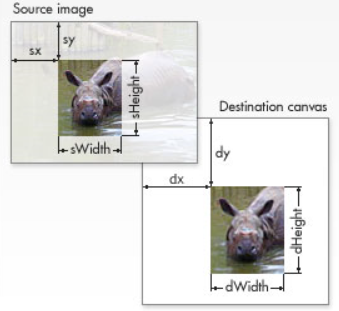
\includegraphics[width=0.3\linewidth]{Figures/ImagenRecorte_Canvas}
  \decoRule
  \caption[Ejemplo recorte imagen canvas.]{Ejemplo recorte imagen canvas.}
   \label{fig:ImagenRecorte_Canvas}
\end{center}
\end{figure}
\end{itemize}
\subsubsection*{Transformaciones}
Antes de indicar las transformaciones disponibles es necesario conocer los métodos \texttt{save()} y \texttt{restore()}. El primero se utiliza para guardar el estado del lienzo antes de aplicar un cambio en el lienzo mientras que el otro se encarga de recuperar el estado del lienzo guardado.
\\Ahora es momento de presentar las distintas transformaciones que se pueden utilizar
\begin{itemize}
\item \texttt{translate(x,y):} Mueve el lienzo y su origen a la coordenada (x,y).
\item\texttt{ rotate(angle):} Gira el lienzo en sentido a las agujas del reloj hasta encontrar el angulo (radianes) indicado.
\item \texttt{scale(x,y):} Escala x e y unidades del lienzo. Se tratan de números reales,si son menores a la unidad disminuyen el tamaño encaso contrario aumentan el tamaño.
\end{itemize}
Se emplea esta etiqueta en el desarrollo de las practicas del ComeCocos Web y del ComeCocos Multijugador.
\subsection{Media}
El nuevo estándar incorpora etiquetas que permiten incorporar contenido multimedia \cite{multimedia} en la web de forma nativa ya que antes era necesario utilizar puglins externos. La etiqueta \textit{<video>} permite incrustar un vídeo en la web e incorpora la posibilidad de establecer múltiple formatos ya que no todos los formatos de vídeo son compatibles en cada uno de los navegador.
\begin{itemize}
    \item Normalmente, un contenedor WebM empaqueta audio Ogg Vorbis con vídeo VP8 / VP9. Esto es soportado principalmente por Firefox y Chrome.
    \item Un contenedor MP4 suele empaquetar audio AAC o MP3 con vídeo H.264. Esto se apoya principalmente en Internet Explorer y Safari.
    \item El contenedor Ogg más antiguo tiende a ir con Ogg Vorbis audio y vídeo Ogg Theora. Esto fue apoyado principalmente en Firefox y Chrome, pero básicamente ha sido reemplazado por el mejor formato WebM. 
\end{itemize}
Las principales características de las que dispone la etiqueta \texttt{<video>} son las siguientes:
\begin{itemize}
  \item\texttt{widtg/height:} Tamaño del vídeo
  \item \texttt{autplay:} Indica que una vez se ha cargado el elemento empiece la reproducción automáticamente.
  \item \texttt{loop:} Se crea un bucle en el que se repite indefinidamente el vídeo.
  \item \texttt{muted:} Desactiva el sonido.
  \item \texttt{poster:} Toma la dirección de una imagen que se muestra antes de empezar la reproducción del vídeo.
  \item \texttt{src:} Contiene la ruta de acceso al vídeo
  \item \texttt{controls:} Permite a los usuarios pausar , reproducir o ajustar el volumen del vídeo.
\end{itemize}
Además tenemos la etiqueta \texttt{<audio>} que permite incrustar audio en la web, en cuanto a su funcionalidad es similar al de la etiqueta \texttt{<video>} aunque no presenta un interfaz gráfico.
\\El primer elementos se emplea en el desarrollo del Sitio Web y Videoconferencia con WebRTC mientras el segundo elemento se emplea en el ComeCocos, ComeCocos Multijugador, Sitio Web y VideoConferencia WebRTC todas las practicas.
omeCocos Web y del ComeCocos Multijugador.
\subsection{WebSockets}
Internet se ha creado a partir del paradigma solicitud/respuesta de HTTP. Un cliente carga una página web, se cierra la conexión y no ocurre nada hasta que el usuario hace click en un enlace o envía un formulario.
\\Hace algún tiempo que existen técnicas que ofrecen al servidor llevar la iniciativa, como por ejemplo Comet. Uno de las técnicas más comunes para crear la ilusión de una conexión iniciada por el servidor se denomina Long Polling. Con el Long Polling, el cliente abre una conexión HTTP con el servidor, el cual la mantiene abierta hasta que se envíe una respuesta. Cada vez que el servidor tenga datos nuevos los enviará como respuesta a cada petición pendiente.
\\La tecnología WebSockets \cite{Websockets} ofrece estas características de modo nativo sin necesidad de utilizar trucos como en caso de Comet permitiendo al servidor llevar la iniciativa sin problemas, figura \ref{fig:websocketsDiag}.
\begin{enumerate}
\item \textbf{Conexión bidireccional:} Esta conexión se produce en tiempo real y se mantiene permanentemente abierta hasta que se cierre de manera explícita.
\item \textbf{Gran rendimiento y escalabilidad:} Si un socket esta abierto, el servidor puede enviar datos a todos los clientes conectados al socket, sin tener que estar constantemente procesando peticiones.
\item \textbf{Latencia:} Como el socket está siempre abierto y escuchando, los datos son enviados inmediatamente desde el servidor al navegador.
\item \textbf{Transmisión de datos:} Los datos a transmitir se reducen también de manera drástica, pasando de un mínimo de 200-300 bytes en peticiones Ajax, a 10-20 bytes.
\end{enumerate}
\begin{figure}[!h]
\begin{center}
   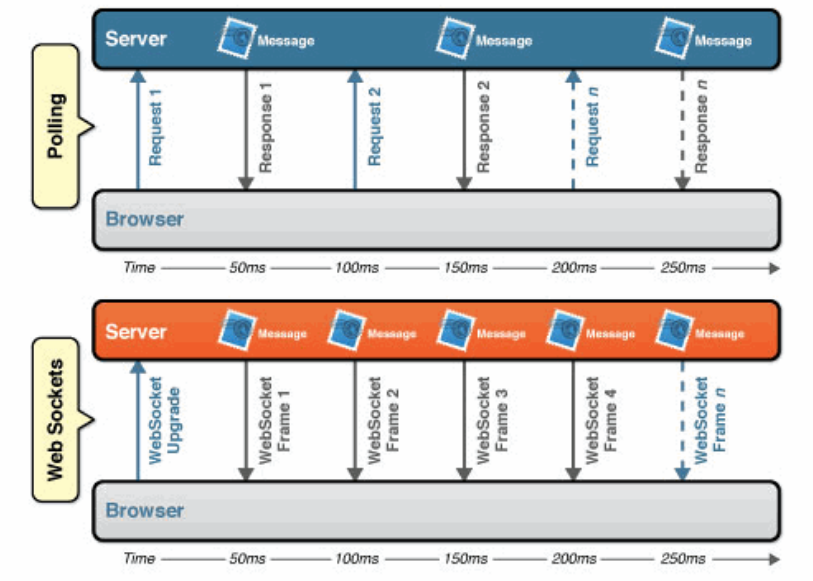
\includegraphics[width=0.7\linewidth]{Figures/websocketsDiag}
  \decoRule
  \caption[Comparación Polling-WebSockets]{Comparación Polling-WebSockets.}
\label{fig:websocketsDiag}
\end{center}
\end{figure}
\subsubsection*{Funcionamiento API}
El cliente establece una conexión WebSockets\cite{WebSocketEjemplo} a través de un proceso conocido como \textit{Handshake WebSocket}. Este proceso se inicia con una solicitud HTTP normal al servidor que incluye el campo \texttt{Upgrade} para informar al servidor que se desea establecer una conexión WebSocket.
\begin{lstlisting}[
caption=Petición conexión WebSockets.]
 GET ws://websocket.example.com/ HTTP/1.1
 Origin: http://example.com
 Connection: Upgrade
 Host: websocket.example.com
 Upgrade: websocket
\end{lstlisting}
Si el servidor soporta el protocolo WebSockets,lo comunica a través del campo \texttt{Upgrade} en la respuesta.
\begin{lstlisting}[
caption=Respuesta conexión WebSockets.]
HTTP/1.1 101 WebSocket Protocol Handshake
Date: Wed, 16 Oct 2013 10:07:34 GMT
Connection: Upgrade
Upgrade: WebSocket
\end{lstlisting}
Ahora que el proceso \textit{Handshake} se ha completado, la conexión inicial de HTTP se sustituye por una conexión WebSockets que utiliza la misma conexión TCP / IP subyacente. En este punto, cualquiera de las partes puede iniciar el envío de datos.
\subsubsection*{Librería Socket.io}
Socket.IO \cite{socketiO} es una librería de JavaScript que facilita el desarrollo de aplicaciones basadas en Websockets tanto en el cliente como en el servidor.
\\En lado servidor(NodeJS) se importa la librería por medio de la sentencia \texttt{require()}
\begin{lstlisting}[
caption=Llamada libreria Socket.IO Server.]
var io = require('socket.io')(server); 
\end{lstlisting}
Para iniciar la conexión WebSockets se emplea el evento \texttt{io.on('connection',function())} 
\begin{lstlisting}[
caption=Comprobación conexión WebSockets Server.]
io.on('connection', function(socket) {  
    console.log('Un cliente se ha conectado');
});
\end{lstlisting}
En el lado cliente es necesario incluir el script \texttt{socket.io.js} en el fichero HTML de proyecto.
\begin{lstlisting}[
caption=Instancia libreria Socket.IO cliente.]
 <script src="/socket.io/socket.io.js"></script> 
\end{lstlisting}
Para establecer la conexión Websocket utilizamos el método \texttt{io.connnect} al que se le pasa la url donde se encuentra el servidor con el que se quiere establecer la conexión.
\begin{lstlisting}[
caption=Llamada libreria Socket.IO cliente.]
 var socket = io.connect('http://localhost:8080');
\end{lstlisting}
Una vez establecida la conexión entre el cliente y servidor pueden enviar mensajes \footnote{https://socket.io/} utilizamos el método \texttt{emit}, que recibe el nombre del mensaje y los datos que se envían. El receptor del mensaje utiliza el método \texttt{on} para definir un evento  con el nombre del mensaje que espera recibir y un \textit{callback} que se encarga de obtener los datos del mensaje.
\begin{lstlisting}[
caption=Ejemplo Envió-Recepción mensaje con WebSockets.]
 //cliente 
 socket.emit('new-message', 'ola');
 
 //server
 socket.on('new-message', function(data) {  
  console.log(data)
 });
\end{lstlisting}
La versión 1.0 de la librería se utiliza en el desarrollo de las practicas del ComeCocos Multijugador y de Videoconferencia con WebRTC.
\subsection{API File}
El tratamiento de ficheros por parte de los navegadores de forma nativa no fue posible hasta la aparición de API File \cite{APIFile}. La API requiere de una etiqueta \texttt{<input>} para seleccionar el archivo con el que se quiere trabajar, a continuación JavaScript se encarga de obtener la información del documento a través del objeto \texttt{FileReader()}.
\begin{lstlisting}[
caption=Ejemplo API File.]
<!DOCTYPE html>
<head>
 <meta charset="utf-8">
 <title>File API</title>
 <script type="text/javascript">
  function processFiles(file){
   var files = file[0];
   var reader = new FileReader();
   reader.onload = function (e) {
    /*
     e.result tiene el resultado de la 
     lectura del fichero
    */
   };
   reader.readAsArrayBuffer(files);
  }
 </script>
</head>
<body>
 Select a text file:
 <input type="file" id="fileInput" onchange="processFiles(this.files)">
</body>
</html>
\end{lstlisting}
Es necesario especificar el modo en el que la API va a leer la información. A continuación se resumen los métodos disponibles:
\begin{itemize}
\item \texttt{reader.readAsText():} Permite leer archivos de texto y recibe dos parámetros. El primer parámetro es el objeto file o Blob que se va a leer y el segundo parámetro se utiliza para especificar la codificación del archivo.
\item \texttt{reader.readAsDataURL():} Permite leer un File o Blob y generar una URL de datos . Esto es básicamente una cadena base64 de los datos del archivo. Se puede utilizar esta URL datos para cosas como el establecimiento de la propiedad \texttt{src} de una imagen.
\item \texttt{reader.readAsBinaryString():} Permite leer cualquier tipo de archivo. El método devuelve los datos binarios sin formato.
\item \texttt{reader.readAsArrayBuffer():} Permite leer un File o Blob y obtener como resultado un ArrayBuffer, es decir,un buffer de datos binarios de longitud fija.
\end{itemize}
Esta API se utiliza en el desarrollo de la practica de Videoconferencia con WebRTC.
\section{JavaScript}
JavaScript \cite{javascript} es un lenguaje de programación interpretado que permite crear script con eventos, clases y acciones para el desarrollo de aplicaciones Internet del lado del cliente. Los usuarios no leerán únicamente las páginas sino que adquieren un carácter interactivo permitiendo cambiar las paginas dentro de una aplicación: poner botones, cuadros de texto, código para hacer una calculadora, un editor de texto, un juego, o cualquier otra cosa.
\subsection*{Propiedades}
\begin{itemize}
\item Se interpreta por el ordenador que recibe el programa, no se compila.
\item Tiene una programación orientada a objetos. El código de los objetos está predefinido y es expandible. No usa clases ni herencia.
\item El código está integrado (incluido) en los documentos HTML.
\item No se declaran los tipos de variables.
\item Ejecución dinámica: los programas y funciones no se chequean hasta que se ejecutan.
\item Parte de los programas de JavaScript se ejecuta cuando sucede un evento. 
\end{itemize}
\section{JQuery}
JQuery \cite{jquery}\cite{jqueryOficial} es un entonro Javascript que sirve como base para la programación avanzada  de aplicaciones del lado del cliente aportando una serie de funciones o códigos para realizar tareas habituales.
\subsection*{Características}
\begin{itemize}
\item efectos dinámicos.
\item aplicaciones que hacen uso de Ajax.
\item manipular el árbol DOM.
\item manejo de eventos.
\item desarrollar animaciones
\item simplifica la manera de interactuar con los documentos HTML
\end{itemize}
La versión 3.2.0 de la librería se emplea en el desarrollo de todas las practicas ya que nos permite simplificar ciertas tareas.
\section{Bootstrap}
Bootstrap \cite{bootstrap}\cite{bootstrapOfi} es un entorno (front-end) de twitter para desarrollo de aplicaciones web. Se basa en un sistema de grid de 12 columnas que escalan adecuadamente a medida que aumenta el tamaño del dispositivo o la ventana de visualización. Además contiene elementos de diseño básicos de HTML y CSS, como pueden ser barras de navegación, plantillas predefinidas, botones,desplegables entre otras extensiones de JavaScript.
\subsection*{Características}
\begin{itemize}
\item Sencillo y ligero
\item Basado en los últimos estándares de desarrollo de Web
\item Curva de aprendizaje baja
\item Compatible con todos los navegadores habituales
\item Responsive web design.
\end{itemize}
La versión 3.3.7 del este entorno se utiliza para diseñar la apariencia de todas las practicas.
\section{NodeJS}
Es un proyecto de software libre creado por Ryan Dahl a principios de 2009  orientado a la creación de aplicaciones para Internet,principalmente Web. La idea empezó a gestarse a partir de otro proyecto para el entorno Ruby on Rails, un pequeño y rápido servidor web llamado Ebb, que evolucionó a una librería en C.
\\Una de las razones de la evolución del proyecto desde Ruby a C, y luego de C a JavaScript fue el objetivo de realizar un sistema en que la Entrada/Salida fuera enteramente no bloqueante que es esencial para obtener un alto rendimiento. Según \cite{nodejs}
{\textit{“Node.js es una plataforma construida encima del entorno de ejecución javascript
de Chrome para fácilmente construir rápidas, escalables aplicaciones de red.
Node.js usa un modelo de E/S no bloqueante dirigido por eventos que lo hace ligero
y eficiente, perfecto para aplicaciones data-intensive en tiempo real”}
\subsection*{Fácil desarrollo y escalabilidad}
Una de las ventajas de emplear JavaScript como lenguaje para las aplicaciones \textit{Node} es que, al tratarse de un lenguaje con una curva de aprendizaje suave permite desarrollar aplicaciones rápidamente con sólo tener unas nociones básicas de las características de este lenguaje.
\\Uno de los aspectos con mayor impacto en cuanto a la escalabilidad es el diseño del sistema. Este es uno de los punto fuertes de \textit{Node} ya que su arquitectura y la forma de desarrollar sus aplicaciones hacen que se cumplan los principios básicos de escalabilidad.
\subsection*{E/S no bloqueante por eventos}
Uno de los puntos críticos es el cuello de botella que afecta en alto grado al rendimiento de cualquier sistema, en especial aquellos que hacen un uso intensivo de operaciones de Entrada/Salida con ficheros y dispositivos. Para solventar este problema \textit{Node} utiliza un modelo de concurrencia basado en eventos que implicar utilizar los siguientes requisitos:
\begin{itemize}
\item Necesidad de un bucle de procesado de eventos que se tratara como un único proceso y que sólo ejecuta un manejador, o \textit{callback}, a la vez.
\item  Emplear un lenguaje que se adapte a este modelo como es el caso de JavaScript ya que su intérprete se basa un modelo idéntico.
\end{itemize}
\subsection*{Ligero y Eficiente}
\textit{Node} es una fina capa de software entre el sistema operativo y la aplicación escrita ya que con su arquitectura se persigue velocidad y eficiencia.
\\Centrado en este propósito descarta emplear un modelo \textit{multihead} para manejar las distintas conexiones ya que el coste es muy elevado. Se busca entonces una solución de alto rendimiento que permita realizar operaciones Entrada/Salida no bloqueantes delegando en el sistema operativo y coordinarlo a través de uno o varios bucles de eventos.
\subsection*{Perfecto para aplicaciones en tiempo real}
\textit{Node} encaja con los requisitos que exigen las aplicaciones en tiempo real flexibles. De acuerdo a su capacidad de manejar un alto número de conexiones y procesar un enorme número de operaciones de Entrada/Salida muy rápido se puede afirmar que \textit{Node} encaja perfectamente si se requiere:
\begin{itemize}
\item \textbf{Interfaces ligeros REST/JSON:} su modelo de Entrada/Salida para atender peticiones \textit{REST} junto al soporte nativo \textit{JSON} lo hacen óptimo como capa superior de fuente de datos como base de datos.
\item \textbf{Aplicaciones monopágina:} la interacción del cliente con el servidor se realiza por medio de peticiones \textit{Ajax}. El uso de \textit{Ajax} puede producir una avalancha de peticiones que el servidor tiene debe ser capaz de procesar es aquí donde \textit{Node} entra en acción.
\item \textbf{Datos por streaming:} al tratarse de conexiones HTTP como streams, permite procesar ficheros al vuelo.
\item \textbf{Comunicación:} aplicaciones de mensajería instantánea o web en tiempo real,e incluso, juegos multijugador.
\end{itemize}
La versión 6.10 se utiliza en el desarrollo del las practicas del ComeCocos Multijugador} y Videoconferencia con WebRTC.
\section{Base de Datos}
El objetivo principal de las BBDD \cite{bbdd} es unificar los datos que se manejan y los programas o aplicaciones que los manejan. Antiguamente los programas se codificaban junto con los datos lo que desembocaba en una dependencia de los programas respecto a los datos. Además, cada aplicación utiliza ficheros que pueden ser comunes a otras sectores de la misma aplicación lo que producía redundancia en la información.

Con las BBDD se busca independizar los datos que residen en memoria y las aplicaciones que manipulan la información mediante un sistema gestor de BBDD. Por lo tanto una base de datos pretende conseguir a través del Sistema Gestor de Bases de Datos(SGBD):
\begin{itemize}
\item \textbf{Independencia de datos:} Cambios en la estructura de la Base de Datos no modifican las aplicaciones.
\item \textbf{Integridad de los datos:} Los datos han de ser siempre correctos. Se establecen una serie de restricciones (reglas de validación) sobre los datos.
\item \textbf{Seguridad de los datos:} Control de acceso a los datos para evitar manipulaciones no deseadas. 
\end{itemize}
\begin{figure}[!h]
\begin{center}
   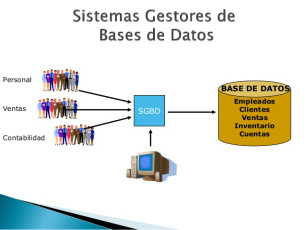
\includegraphics[width=0.5\linewidth]{Figures/BBDD_Esquema}
  \decoRule
  \caption[Esquema Base de Datos.]{Esquema Base de Datos.}
\label{fig:BBDD_Esquema}
\end{center}
\end{figure}
\subsection{MySQL}
Es un sistema de administración de bases de datos relacionales almacenando los datos en tablas separadas en lugar de poner todos los datos en un solo lugar. Esto agrega velocidad y flexibilidad.
\\Para procesar acciones existen las siguientes sentencias básicas para trabajar con este gestor de bases de datos.
\begin{enumerate}
\item \textbf{Uso BBDD:} La sentencia \texttt{USE nombreBd} permite seleccionar la BBDD con la que se quiere trabajar.
\item \textbf{Visualización:} Para ver todas las BBDD se utiliza la sentencia \texttt{SHOW DATABASES} mientras que para las tablas de una BBDD se utiliza \texttt{SHOW TABLES}.
\item \textbf{Búsqueda:} Una de las sentencias de este tipo es \texttt{SELECT * FROM nombreTabla} que permite visualizar el contenido de una determinada tabla.
\item \textbf{Crear y Eliminar:} La sentencia \texttt{CREATE DATABASE nombreBd} crea y la sentencia \texttt{DROP DATABASE nombreBd} elimina una BBDD.
\end{enumerate}
La versión 5.0 se ha utilizado para desarrollar la practica Sitio Web de una tienda.
\section{Django}
Consideremos el diseño de una aplicación Web escrita usando el estándar Common Gateway Interface (CGI), una forma popular de escribir aplicaciones Web en el año 1998. En esa época, cuando escribías una aplicación CGI se desarrollaba todas las tareas por uno mismo. Este enfoque es valido si la aplicación solo utiliza un fichero pero a medida que una aplicación Web crece aparecen una serie de problemas:
\begin{itemize}
\item ¿Qué sucede cuando múltiples páginas necesitan conectarse a la BBDD? El código de conexión a la BBDD no debería estar en cada uno de los script ya que la mejor forma de hacerlo es refactorizarlo en una función compartida.
\item ¿Qué sucede cuando este código es reutilizado en múltiples entornos, con BBDD y contraseñas diferentes? En ese punto, se vuelve esencial alguna configuración específica del entorno.
\item ¿Qué sucede cuando un diseñador Web no tiene experiencia programando y desea rediseñar la página? Lo ideal sería que la lógica de la página esté separada del código HTML de la página.
\end{itemize}
Precisamente estos son los problemas que un entorno Web intenta resolver por medio de una infraestructura de programación para las aplicaciones permitiendo escribir código limpio y de fácil mantenimiento. En nuestro caso utilizamos Django \cite{django}.
\subsection{Diseño MVC en Django}
El diseño general de este entorno esta compuesto de tres partes que se detallan a continuación.
\subsubsection*{Models}
Los modelos se representan como una clase Python dentro del fichero \textit{models.py} en el que se define cada uno de los elementos por medio del el objeto \texttt{models}\footnote{fuente: \url{https://docs.djangoproject.com/en/1.10/ref/models/fields/}}.
\begin{lstlisting}[
language=Python,
caption=Ejemplo de un Modelo.]
 from django.db import models
 class Artista(models.Model):
  name = models.CharField(max_length=100,null=True)
  videos = models.ManyToManyField(Videos) 
  galeria = models.ManyToManyField(Imagenes)
\end{lstlisting}
Además existe la posibilidad de establecer relación entre las distintas clases del fichero por medio de los siguiente métodos:
\begin{itemize}
\item \textbf{models.ForeignKey:} relación 1 a 1.
\item\textbf{ models.ManyToManyField:} relación 1 a n.
\end{itemize}
Tras migrar la información del fichero se genera tantas tablas como clases existan.
\subsubsection*{Vistas}
Una vista es una función en Python que contiene la lógica para interactuar con la BBDD definida dentro del fichero \textit{view.py}. Para obtener la información Django permite emplear filtro definidos en Python sin necesidad de programar en SQL.
\begin{lstlisting}[
language=Python,
caption=Ejemplo de vistas.]
 from django.http import HttpResponse 
 def EventSelect(request,evento):
  event = Evento.objects.filter(name__startswith=evento)
  return render(request,'IndexEvent.html',{'event':event})
 def IndexView(request):
  list_video=Videos.objects.all()
  return render(request,'fullVideo.html',{'list_video':list_video})
\end{lstlisting}
Las funciones se pueden dividir en dos grupos:
\begin{itemize}
\item \textbf{Dinámicas:} Son aquellas que reciben el parámetro \texttt{request} y un parámetro adicional a través de la url.
\item \textbf{Estáticas:} Son aquellas que reciben solo el parámetro \texttt{request}.
\end{itemize}
\subsubsection*{Controlador}
Un controlador se representa como una dupla en Python dentro del fichero \textit{urls.py} que define las distintas rutas de acceso a la aplicación y la vista asociada.
\begin{lstlisting}[
language=Python,
caption=Ejemplo de url's.]
 # urls.py 
 from django.conf.urls.defaults import patterns, url
 from .views import ....
 urlpatterns = patterns('',
  url(r'^index/$',  views.MainPage),
  url(r'^eventos/(?P<evento>\w{1,50})/$',  views.EventSelect),
 )
\end{lstlisting}
Al igual que en las vistas las URLs pueden ser de dos tipos:
\begin{itemize}
\item \textbf{Dinámicas:} El path esta formado por texto y un parámetro adiciona.
\item \textbf{Estáticas:} El path se define como una cadena de texto.
\end{itemize}
\subsubsection*{Plantilla}
Una plantilla es un fichero html enriquecido con un lenguaje de etiquetas adicional que permite renderizar la información enviadas por la vista correspondiente. Para plasmar esta información utilizamos el lenguaje de plantillas\footnote{\url{https://docs.djangoproject.com/en/1.10/ref/templates/}} que es similar a un lenguaje de programación ya que posee bucles, variables de plantillas asociadas a variables Python, sentencias condicionales entre otras características.
\begin{lstlisting}[
language=HTML,
caption=Ejemplo de plantilla.]
 <!DOCTYPE html>
 <html>
  <head>
  </head>
  <body>
    <p>Dia y hora actual: {{fechahora\_actual}}</p>
    
    <p>{{cantante.name}}</p>
     </div>
    
    
  </body>    
</html>
\end{lstlisting}
 El lenguaje de plantillas define los siguientes modos de acceso a la información:
\begin{itemize}
\item El contenido entre \textbf{\{\{ \}\}} muestra el valor de una variable de plantilla.
\item El contenido entre \textbf{\{\% \%\}} hace referencia a las etiquetas del lenguaje de plantilla.
\item Se puede establecer un bloque a través de la etiqueta \textbf{\{\% block nameseccion \%\}} y \textbf{\{\% endblock \%\}} que se utilizan al establecer herencia entre las plantillas.
\end{itemize}
Estas piezas relacionadas en conjunto se aproximan al patrón Modelo-Vista-Controlador(MVC). Este patrón permite el código que interactúa con los datos (modelo) esté separado de la asignación de rutas (controlador) y a su vez separado del interfaz del usuario (vista).
\\La principal ventaja de este enfoque es el acoplamiento débil entre sí, es decir, cada pieza de la aplicación Web tiene un único propósito por lo que puede ser modificado independientemente sin afectar a las otras piezas.
\begin{figure}[!h]
\begin{center}
   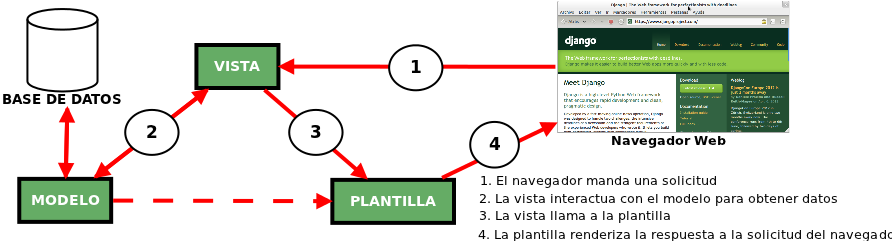
\includegraphics[width=0.85\linewidth]{Figures/esquemaDjango}
  \decoRule
  \caption[Esquema MVC Django.]{Esquema MVC Django.}
\label{fig:esquemaDjango}
\end{center}
\end{figure}

La versión 1.9 de este frameWork se utiliza para desarrollar la practica de Sitio Web de una tienda.
\section{WebRTC}
WebRTC es una tecnología soportada por el W3C (World Wide Web Consortium) que permite establecer comunicación \textit{peer-to-peer} entre los navegadores Web e intercambiar audio, vídeos o archivos.

Para construir una aplicación de este tipo desde cero, seria necesario una gran cantidad bibliotecas que se ocupan de problemas típicos como la pérdida de datos, caída de conexiones y atravesamiento de NATs pero WebRTC \cite{webRTC} incorpora de forma nativa las soluciones a estos problemas.
\subsection*{MediaStream APIs}
Es una API diseñada para acceder fácilmente a los flujos de datos de las cámaras y micrófonos desde el navegador web. El método \texttt{getUserMedia()} es la forma principal para acceder al flujo de datos de los dispositivos.
La API posee las siguientes características:
\begin{enumerate}
\item Un flujo de \textit{stream} en tiempo real está representado por un objeto \textit{stream} en forma de vídeo o audio.
\item Proporciona un nivel de seguridad ya que pide permiso a los usuarios humanos acceso a los elementos multimedia locales.
\end{enumerate}
\subsection*{RTCPeerConection APIs}
RTCPeerConection es el núcleo de la conexión peer-to-peer entre cada uno de los navegadores. Para crear el objeto \texttt{RTCPeerConnection} se realiza la siguiente llamada.
\begin{lstlisting}[
caption=Instancia RTCPeerConnection.]
 var pc = new RTCPeerConnection(config);
\end{lstlisting}
Donde el argumento \texttt{config} contiene al menos la clave, iceServers, que es una matriz de objetos URL que contiene información sobre los servidores STUN y TURN utilizados durante la búsqueda de los candidatos ICE.
\subsubsection*{Propiedades}
\begin{enumerate}
  \item \texttt{RTCPeerConnection.localDescription(read only):} Devuelve un objeto RTCSessionDescription que describe la sesión local.
  \item \texttt{RTCPeerConnection.remoteDescription(read only):} Devuelve un objeto RTCSessionDescription que describe la sesión remota.
\end{enumerate}
\subsubsection*{Controladores de eventos}
\begin{enumerate}
  \item \texttt{RTCPeerConnection.onaddstream:} Se activa cada vez que se añade un objeto MediaStream por el par remoto.
  \item \texttt{RTCPeerConnection.ondatachannel:} Se activa cuando se incluye el canal de datos en el par remoto.
  \item \texttt{RTCPeerConnection.onicecandidate:} Se activa cuando se agrega un objeto RTCIceCandidate.
  \item \texttt{RTCPeerConnection.onremovestream:} Se activa cuando se quita un objeto MediaStream de la conexión.
\end{enumerate}
\subsubsection*{Métodos}
\begin{enumerate}
  \item \texttt{RTCPeerConnection():} Devuelve un nuevo objeto evento \texttt{RTCPeerConnection}.
  \item \texttt{RTCPeerConnection.createOffert(HandlerOffert,HandlerError,Options):} Crea una solicitud de oferta para encontrar un peer remoto. Los dos primeros parámetros de este método son los retornos de la función de éxito y error. El tercer parámetro es opcional.
  \item \texttt{RTCPeerConnection.createAnswer(HandlerAnswer,HandlerError,Options):} Crea una respuesta a la oferta recibida por el peer remoto durante el proceso de negociación (oferta/respuesta). Los dos primeros parámetros de este método son los retornos de la función de éxito y error. El tercer parámetro es opcional.
  \item \texttt{RTCPeerConnection.setLocalDescription():} Cambia la descripción de la conexión local.El método toma tres parámetros, el objeto RTCSessionDescription y los retornos de la función de éxito y fallo.
  \item \texttt{RTCPeerConnection.setRemoteDescription():} Cambia la descripción de la conexión remota.El método toma tres parámetros, el objeto RTCSessionDescription y los retornos de la función de éxito y fallo.
  \item \texttt{RTCPeerConnection.addStream():} Añade un objeto MediaStream como una fuente local de vídeo o audio.
  \item \texttt{RTCPeerConnection.addIceCandidate():} proporciona un candidato remoto al agente ICE.
  \item \texttt{RTCPeerConnection.createDataChannel():} crea un nuevo objeto RTCDataChannel.
  \item \texttt{RTCPeerConnection.close():} finaliza la conexion.
\end{enumerate}
\subsection*{RTCDataChannel APIs}
WebRTC no sólo es bueno para transferir secuencias de audio y video, sino cualquier dato genérico que tengamos. Aquí es donde entra en juego el objeto \texttt{RTCDataChannel}.
\subsubsection*{Propiedades}
\begin{enumerate}
\item \texttt{RTCDataChannel.label(read only):} Devuelve el nombre del canal de datos.
\item \texttt{RTCDataChannel.protocol(read only):} Devuelve una cadena con el nombre de subprotocolo utilizado para este canal.
\item \texttt{RTCDataChannel.label(read only):} Devuelve el estado de la conexión. Los posibles valores:
  \begin{itemize}
    \item connecting: Indica que la conexión aún no está activa.
    \item open: Indica que la conexión se está ejecutando
    \item connecting: Indica que la conexión no se pudo establecer o se ha cerrado
  \end{itemize}
\end{enumerate}
\subsubsection*{Controladores de eventos}
\begin{enumerate}
\item \texttt{RTCDataChannel.onopen:} Se activa cuando se ha establecido la conexión de datos.
\item \texttt{RTCDataChannel.onmessage:} Se activa cuando está disponible un mensaje en el canal de datos.
\item \texttt{RTCDataChannel.onclose:} Se activa cuando la conexión se ha cerrado.
\item \texttt{RTCDataChannel.onerror:} Se activa cuando se produce un fallo.
\end{enumerate}
\subsubsection*{Métodos}
\begin{enumerate}
\item \texttt{RTCDataChannel.close():} Cierra el canal de datos.
\item \texttt{RTCDataChannel.send():} Envía los datos pasados como parámetro a través del canal. Los datos pueden ser blob, cadenas de texto, un ArrayBuffer o un ArrayBufferView.
\end{enumerate}
\subsection*{Servidor Señalización}
Para conectarse con otro usuario debe saber la dirección IP de su dispositivo. Como se ha mencionado anteriormente de esta tarea se encarga \texttt{RTCPeerConnection}. Tan pronto como los dispositivos saben encontrarse a través de Internet, comienza el intercambio de datos sobre qué protocolos y códecs soporta cada dispositivo. Este proceso recibe el nombre señalización que sigue el esquema de la figura \ref{fig:procesoSenalizacion}. 
\begin{figure}[!h]
\begin{center}
   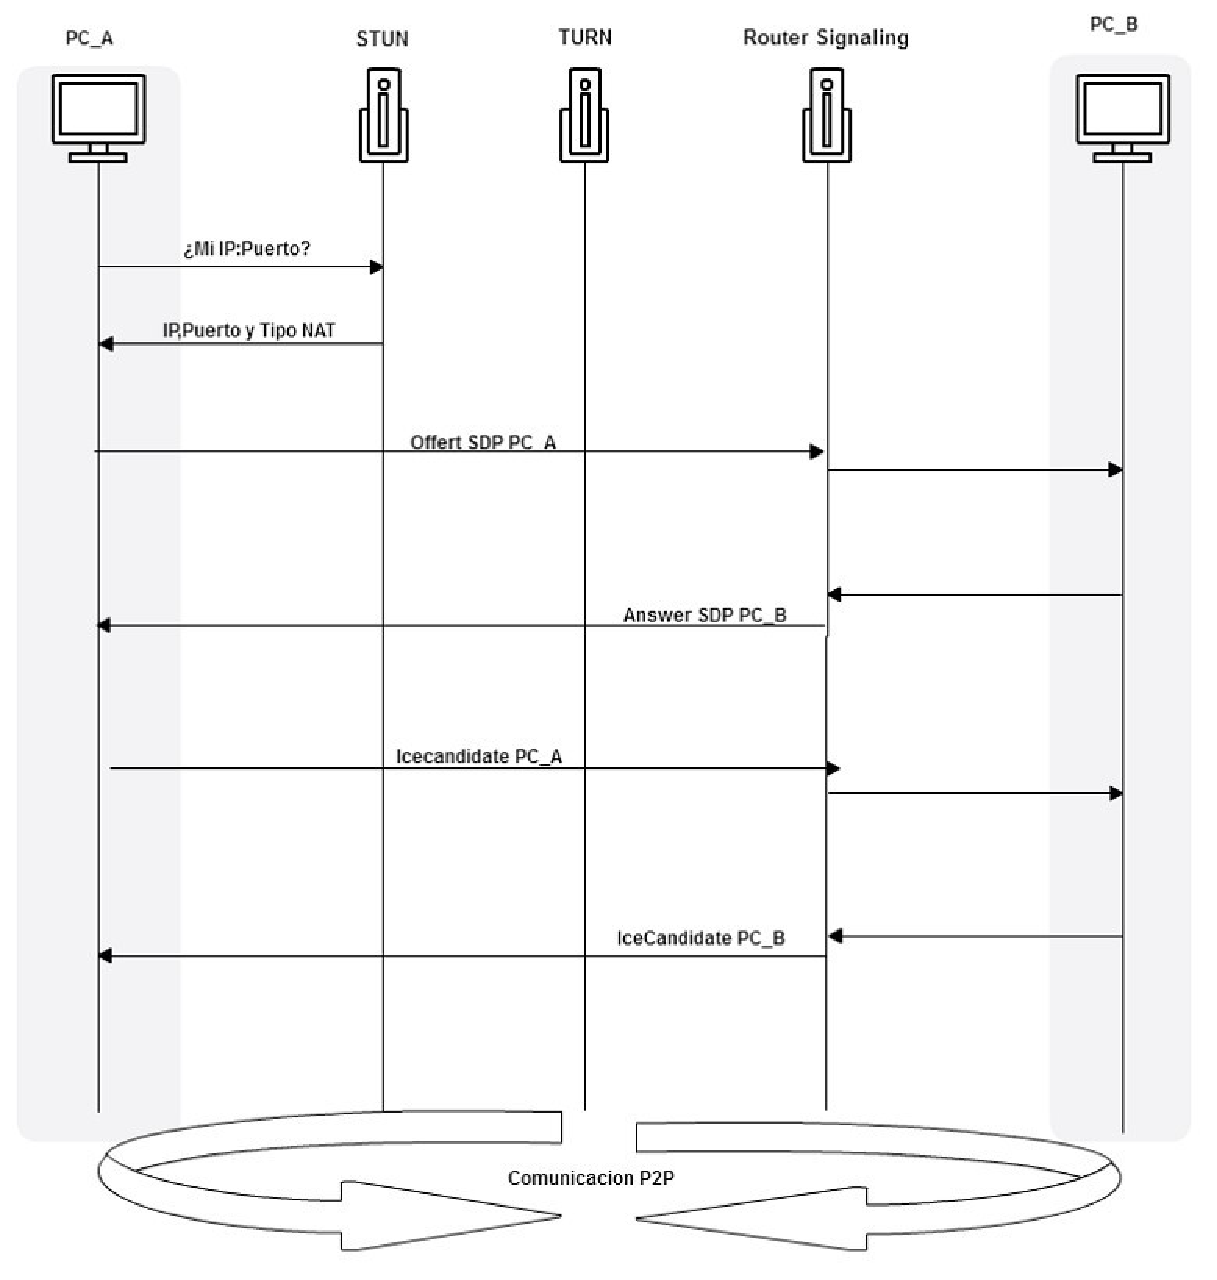
\includegraphics[width=0.7\linewidth]{Figures/procesoSenalizacion}
  \decoRule
  \caption[Proceso del Servidor Señalización]{Proceso del Servidor Señalización.}
\label{fig:procesoSenalizacion}
\end{center}
\end{figure}

En la siguiente lista se explican los pasos de este proceso:
\begin{enumerate}
\item Crea una lista de candidatos potenciales para una conexión entre iguales.
\item El usuario o una aplicación selecciona un usuario con el que establecer una conexión enviando un mensaje que contiene la descripción de la sesión de comunicación (SDP). Este proceso recibe el nombre de Oferta.
\item La capa de señalización notifica el mensaje al otro usuario.
\item Al recibir la oferta el usuario contrario genera un mensaje con su descripción de sesión. Este proceso recibe el nombre de Respuesta.
\item Ambos usuarios guardan el mensaje SDP dentro de su objeto \texttt{RTCPeerConnection} como una descripción de sesión remota.
\item Además ambos usuarios intercambian información de ubicación por medio de los ICECandidate.
\item Finalmente la conexión se establece con  éxito o falla.
\end{enumerate}
La especificación de WebRTC no define ningún estándar sobre el intercambio de información, así que se puede  utilizar cualquier protocolo o tecnología para crear el servidor de señalización. En las siguiente sección explicamos los protocolos que a día de hoy se utilizan con mayor afluencia.

\subsubsection*{SDP}
SDP (Session Description Protocol) es una parte importante del WebRTC. Se trata de un protocolo utilizado para describir las sesiones de comunicación que no entrega los datos de los medios sino que se utiliza para la negociación de codecs de audio y vídeo, topologías de red y otra información de los dispositivos. Se puede definir SDP como una cadena de datos que contiene conjuntos de pares clave-valor, separados por saltos de línea: \texttt{Key = value} como se puede ver en la figura \ref{fig:DescripcionSDP}.
\begin{figure}[!h]
\begin{center}
   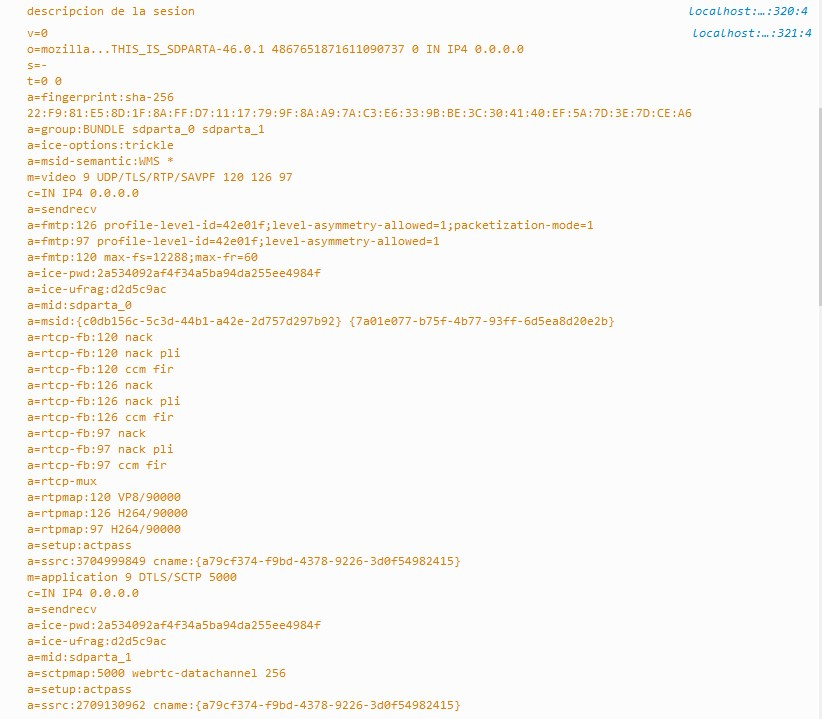
\includegraphics[width=0.9\linewidth]{Figures/DescripcionSDP}
  \decoRule
  \caption[Ejemplo Protocolo SDP]{Ejemplo Protocolo SDP.}
\label{fig:DescripcionSDP}
\end{center}
\end{figure}
%SDP es un método bien conocido para establecer conexiones con los medios de comunicación de los 90s. Se ha utilizado en una gran cantidad de aplicaciones antes de WebRTC como teléfono y conversaciones basadas en texto.%

Este protocolo es la primera parte de la conexión entre pares ya que dicha información se tiene que intercambiar por medio del canal de señalización para finalmente establecer la conexión.
\subsubsection*{STUN}
STUN (Session Traversal Utilities for NAT) ayuda a identificar a cada participante de una comunicación WebRTC y encontrar una buena conexión entre ellos siguiendo los pasos del esquema de la figura \ref{fig:STUN_Example}. En primer lugar realiza una solicitud a un servidor, habilitado con el protocolo STUN, el cual devuelve la dirección IP del cliente. Con esta dirección IP el cliente ahora puede identificarse para establecer conexión.
\begin{figure}[!h]
\begin{center}
   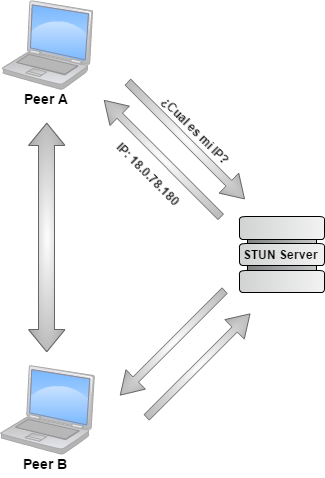
\includegraphics[width=0.3\linewidth]{Figures/TURN_Example}
  \decoRule
  \caption[Ejemplo petición-respuesta STUN]{Ejemplo petición-respuesta STUN.}
\label{fig:STUN_Example}
\end{center}
\end{figure}
\subsubsection*{TURN}
En ocasiones hay cortafuegos que no permite ningún tráfico basado en STUN entre pares. Aquí es donde TURN (Traversal Using Relays around NAT) sale como un método diferente de conectar con otro usuario.

TURN funciona como intermediario entre los clientes ya que obtiene y redirige cada paquete de datos que se envía a él a cada usuario como se ve en la figura \ref{fig:TURN_Example}
\begin{figure}[!h]
\begin{center}
   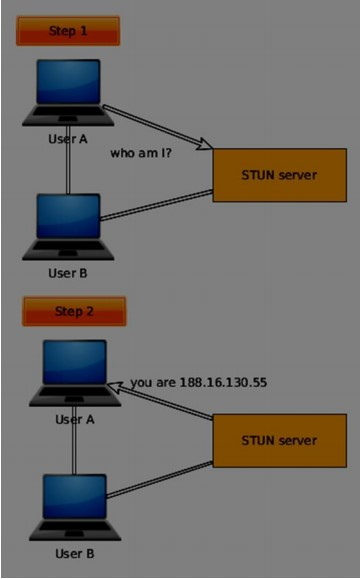
\includegraphics[width=0.3\linewidth]{Figures/STUN_Example}
  \decoRule
  \caption[Ejemplo petición-respuesta TURN]{Ejemplo petición-respuesta TURN.}
\label{fig:TURN_Example}
\end{center}
\end{figure}
\subsubsection*{ICE}
STUN y TURN se unen a través de ICE (Interactive Connectivity Establishment) para proporcionar entre pares exitosa. ICE encuentra y prueba en orden un rango de direcciones que funcionarán para ambos usuarios. Al empezar no sabe nada sobre la red de cada usuario por lo que a través de un conjunto de etapas de forma incremental descubre cómo se configura la red de cada cliente. La tarea principal es encontrar suficiente información de cada red para poder tener éxito en la conexión.
\\STUN y TURN se usan para encontrar cada candidato de ICE por medio del servidor STUN encuentra una IP externa que en caso de fallar pasa a utilizar TURN.
\subsubsection*{SCTP}
Tras establecer la conexión, tenemos la capacidad de enviar rápidamente datos de vídeo y audio. El protocolo SCTP (Stream Control Transmission Protocol) se utiliza para enviar datos (blob) en la parte superior de nuestra conexión al utilizar el objeto \texttt{RTCDataChannel}. Se basa en el protocolo DTLS (Datagram Transport Layer Security) situado encima del protocolo UDP que es el protocolo de transporte base para todas las aplicaciones WebRTC.
\begin{figure}[!h]
\begin{center}
   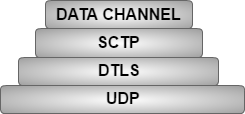
\includegraphics[width=0.4\linewidth]{Figures/SCTP_Example}
  \decoRule
  \caption[Capas de SCTP]{Capas de SCTP.}
\label{fig:SCTP_Example}
\end{center}
\end{figure}

Los desarrolladores de WebRTC sabían que cada aplicación sería única al usar el canal de datos. Algunos podrían querer el alto rendimiento de UDP, mientras que otros pueden necesitar la entrega fiable de TCP. Es por eso que se creó el protocolo SCTP que posee las siguientes características:
\begin{itemize}
\item Existen dos modos de transporte: fiable y no fiable.
\item La capa de transporte está protegida
\item Cuando se transportan mensajes de datos, se permite que se descompongan y vuelvan a montarse en el otro lado.
\item El control del flujo y de la congestión se proporciona a través de la capa de transporte.
\end{itemize}
Se utiliza la versión 1.0 en el desarrollo de la practica de Videoconferencia con WebRTC.
\section{Web Services}
Es un estándar de comunicación entre procesos diseñado para ser multiplataforma y multilenguaje, es decir, no importa el lenguaje ni plataforma donde se ejecute el \textit{Web Services} \cite{webservices}
\\Antiguamente se utilizaban estándares como DCOM \textit{(Distrinuted Component Object Model)} y CORBA (Common Object Request Broker Architecture). Estos estándares presentaban graves problemas de configuración en entornos con cortafuegos ya que era imposible habilitar cierto puertos por temas de seguridad. Por lo que se prefería utilizar el puerto 80 de \textit{HTTP}, que normalmente se encontraba habilitado debido al uso de navegadores y servidores Web. De esta forma HTPP se convirtió en el protocolo preferido para el transporte de mensajes de los \textit{Web Services}.
\subsection*{Características}
\begin{enumerate}
\item \textbf{Combinación:} Las operaciones de un servicio web pueden utilizar otros servicios web para sus operaciones.
\item \textbf{Patrones de comunicación}
  \begin{itemize}
    \item \textbf{Petición-respuesta síncrona:} Invocamos al servicio y esperamos la respuesta a la petición.
    \item \textbf{Comunicación asíncrona:} Se envía la petición y se continúa la ejecución.
    \item \textbf{Mediante eventos:} El cliente se suscribe a eventos ofrecidos por el servicio.
  \end{itemize}
\item \textbf{Desacoplamiento:} Se refiere a minimizar las dependencias entre los servicios para ofrecer una mayor flexibilidad en la arquitectura.
\item \textbf{Representación de mensajes}
  \begin{itemize}
    \item \textbf{Textual:} SOAP representa los servicios y los mensajes en XML.
    \item \textbf{Binario:} Los datos ocupan menos espacio aunque son ilegibles.
  \end{itemize}
\item \textbf{Referencia y activación del servicio:} Los servicios se referencian generalmente mediante una URL, que se conoce como punto final (endpoint). El servicio Web puede ejecutarse en la máquina de punto final, o en servidores secundarios.
\item \textbf{Transparencia:} Protege al programador de los detalles de la representación
de los datos y asemeja una petición local a una remota.
\end{enumerate}
\subsection*{Tipos WebServices}
\textbf{SOAP} \cite{tipoWebServices} (Simple Object Access Protocol) es el protocolo base de los Web Services. Este protocolo esta basado en XML y no se encuentra atado a ninguna plataforma o lenguaje de programación. Si bien es un protocolo, este no es un protocolo de comunicación entre mensajes como lo es HTTP. Básicamente SOAP son documentos XML que necesitan utilizar algún otro protocolo para la ser transmitidos como puede ser HTTP o cualquier otro tipo de protocolo.
Consta de tres componentes principales:
\begin{enumerate}
  \item \textbf{WSDL:} lenguaje de descripción del servicio.
  \item \textbf{HTTP/SMTP:} protocolo de comunicación.
  \item \textbf{XML: }lenguaje de peticiones y respuestas.
\end{enumerate}
\textbf{REST}(Representational State Transfer) intentan emular al protocolo HTTP o protocolos similares mediante la restricción de establecer el interfaz en un conjunto conocido de operaciones estándar (por ejemplo GET, PUT,…). Este estilo se centra más en interactuar con recursos con estado, que con mensajes y operaciones.  
\\Cabe destacar que REST no es un estándar, ya que es tan solo un estilo de arquitectura.
Aunque REST no es un estándar, está basado en estándares:
\begin{itemize}
\item HTTP
\item URL
\item Representación de los recursos: XML/HTML/GIF/JPEG/…
\item Tipos MIME: text/xml, text/html, … 
\end{itemize}
\begin{figure}[!h]
\begin{center}
   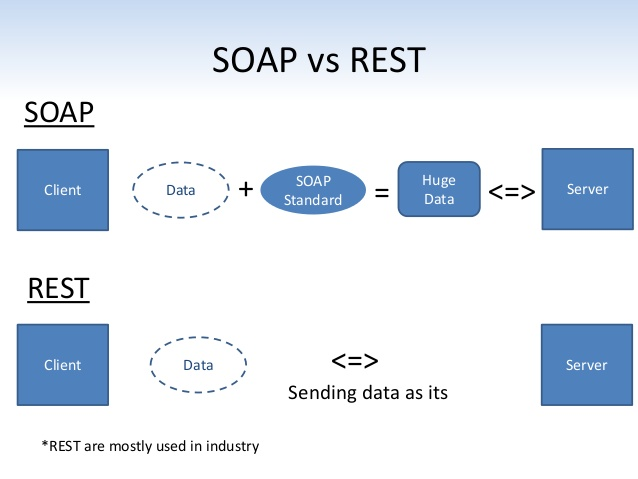
\includegraphics[width=0.5\linewidth]{Figures/Soap_Rest}
  \decoRule
  \caption[Comparativa Soap y Rest]{Comparativa Soap y Rest.}
\label{fig:Soap_Rest}
\end{center}
\end{figure}
\subsection{WebServices Google Maps}
En el desarrollo de la practica Sitio Web de una tienda se ha usaso el WebServices de Google Maps \footnote{Descripción WebServices: https://developers.google.com/maps/web-services/overview} que sigue la estructura REST. Consta de un conjunto de interfaces HTTP que proporcionan datos geográficos para aplicaciones que utilizan mapas.
\\Antes de establecer la comunicación con el WebServices es necesario obtener una clave \footnote{https://developers.google.com/maps/documentation/geocode/get-api-key} asociado a la aplicación que implementa las peticiones. De los numerosos servicios de los que dispone nos centramos en utilizar dos.
\begin{enumerate}
\item \textbf{Geocode \footnote{Descripción API Geocode :https://developers.google.com/maps/documentation/geocoding/}:} permite conocer las coordenadas geograficas de un lugar a partir del nombre. La petición se realiza a la URl definida  en la que se incluye el formato de de los datos(json o xml), el dato que se envía y la clave asociada a la aplicación.
  \begin{lstlisting}[
  caption=Instancia RTCPeerConnection.]
   https://maps.googleapis.com/maps/api/geocode/json?address=Madrid&key=YOUR_API_KEY
  \end{lstlisting}
 \item \textbf{Place \footnote{Descripción API Place :https://developers.google.com/places/web-service/search}:} permite obtener información asociada a un servicio (hoteles,restaurante,...) tomando como punto de referencia una coordenada geográfica. La petición se realiza a la URl definida en la que se incluye el formato de de los datos(json o xml),el dato que se envía y la clave asociada a la aplicación.
\begin{lstlisting}[
caption=Instancia RTCPeerConnection.]
https://maps.googleapis.com/maps/api/place/nearbysearch/json?location=-33.8670,151.1957&radius=500&types=food&key=YOUR_API_KEY
\end{lstlisting}
\section{Inteligencia Artificial}
\end{enumerate} 